\section{Results \& analysis}
\begin{figure}[h]
  \centering
  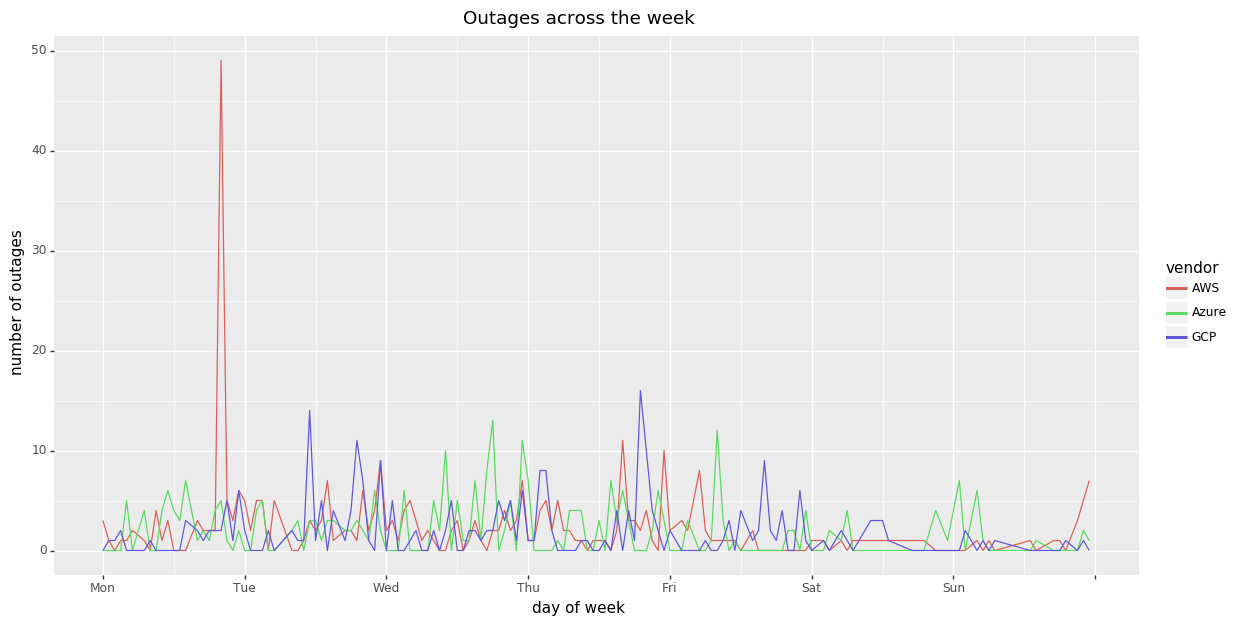
\includegraphics[scale=0.5]{outages-across-week.png}
  \caption{Distribution of outages across the week, by vendor.}
  \label{fig:outages across week}
\end{figure}

We first observe the distribution of outages across the week, this is shown in \autoref{fig:outages across week}.
GCP and AWS both display significant peaks at two points during the week: around the middle (Tuesday and Wednesday), and at the start of the weekend (Friday and Saturday).
AWS also shows an increase in outages in the afternoon/evening hours on Sunday.
The data provided by Azure does not indicate any clear trends.

\begin{figure}[h]
  \centering
  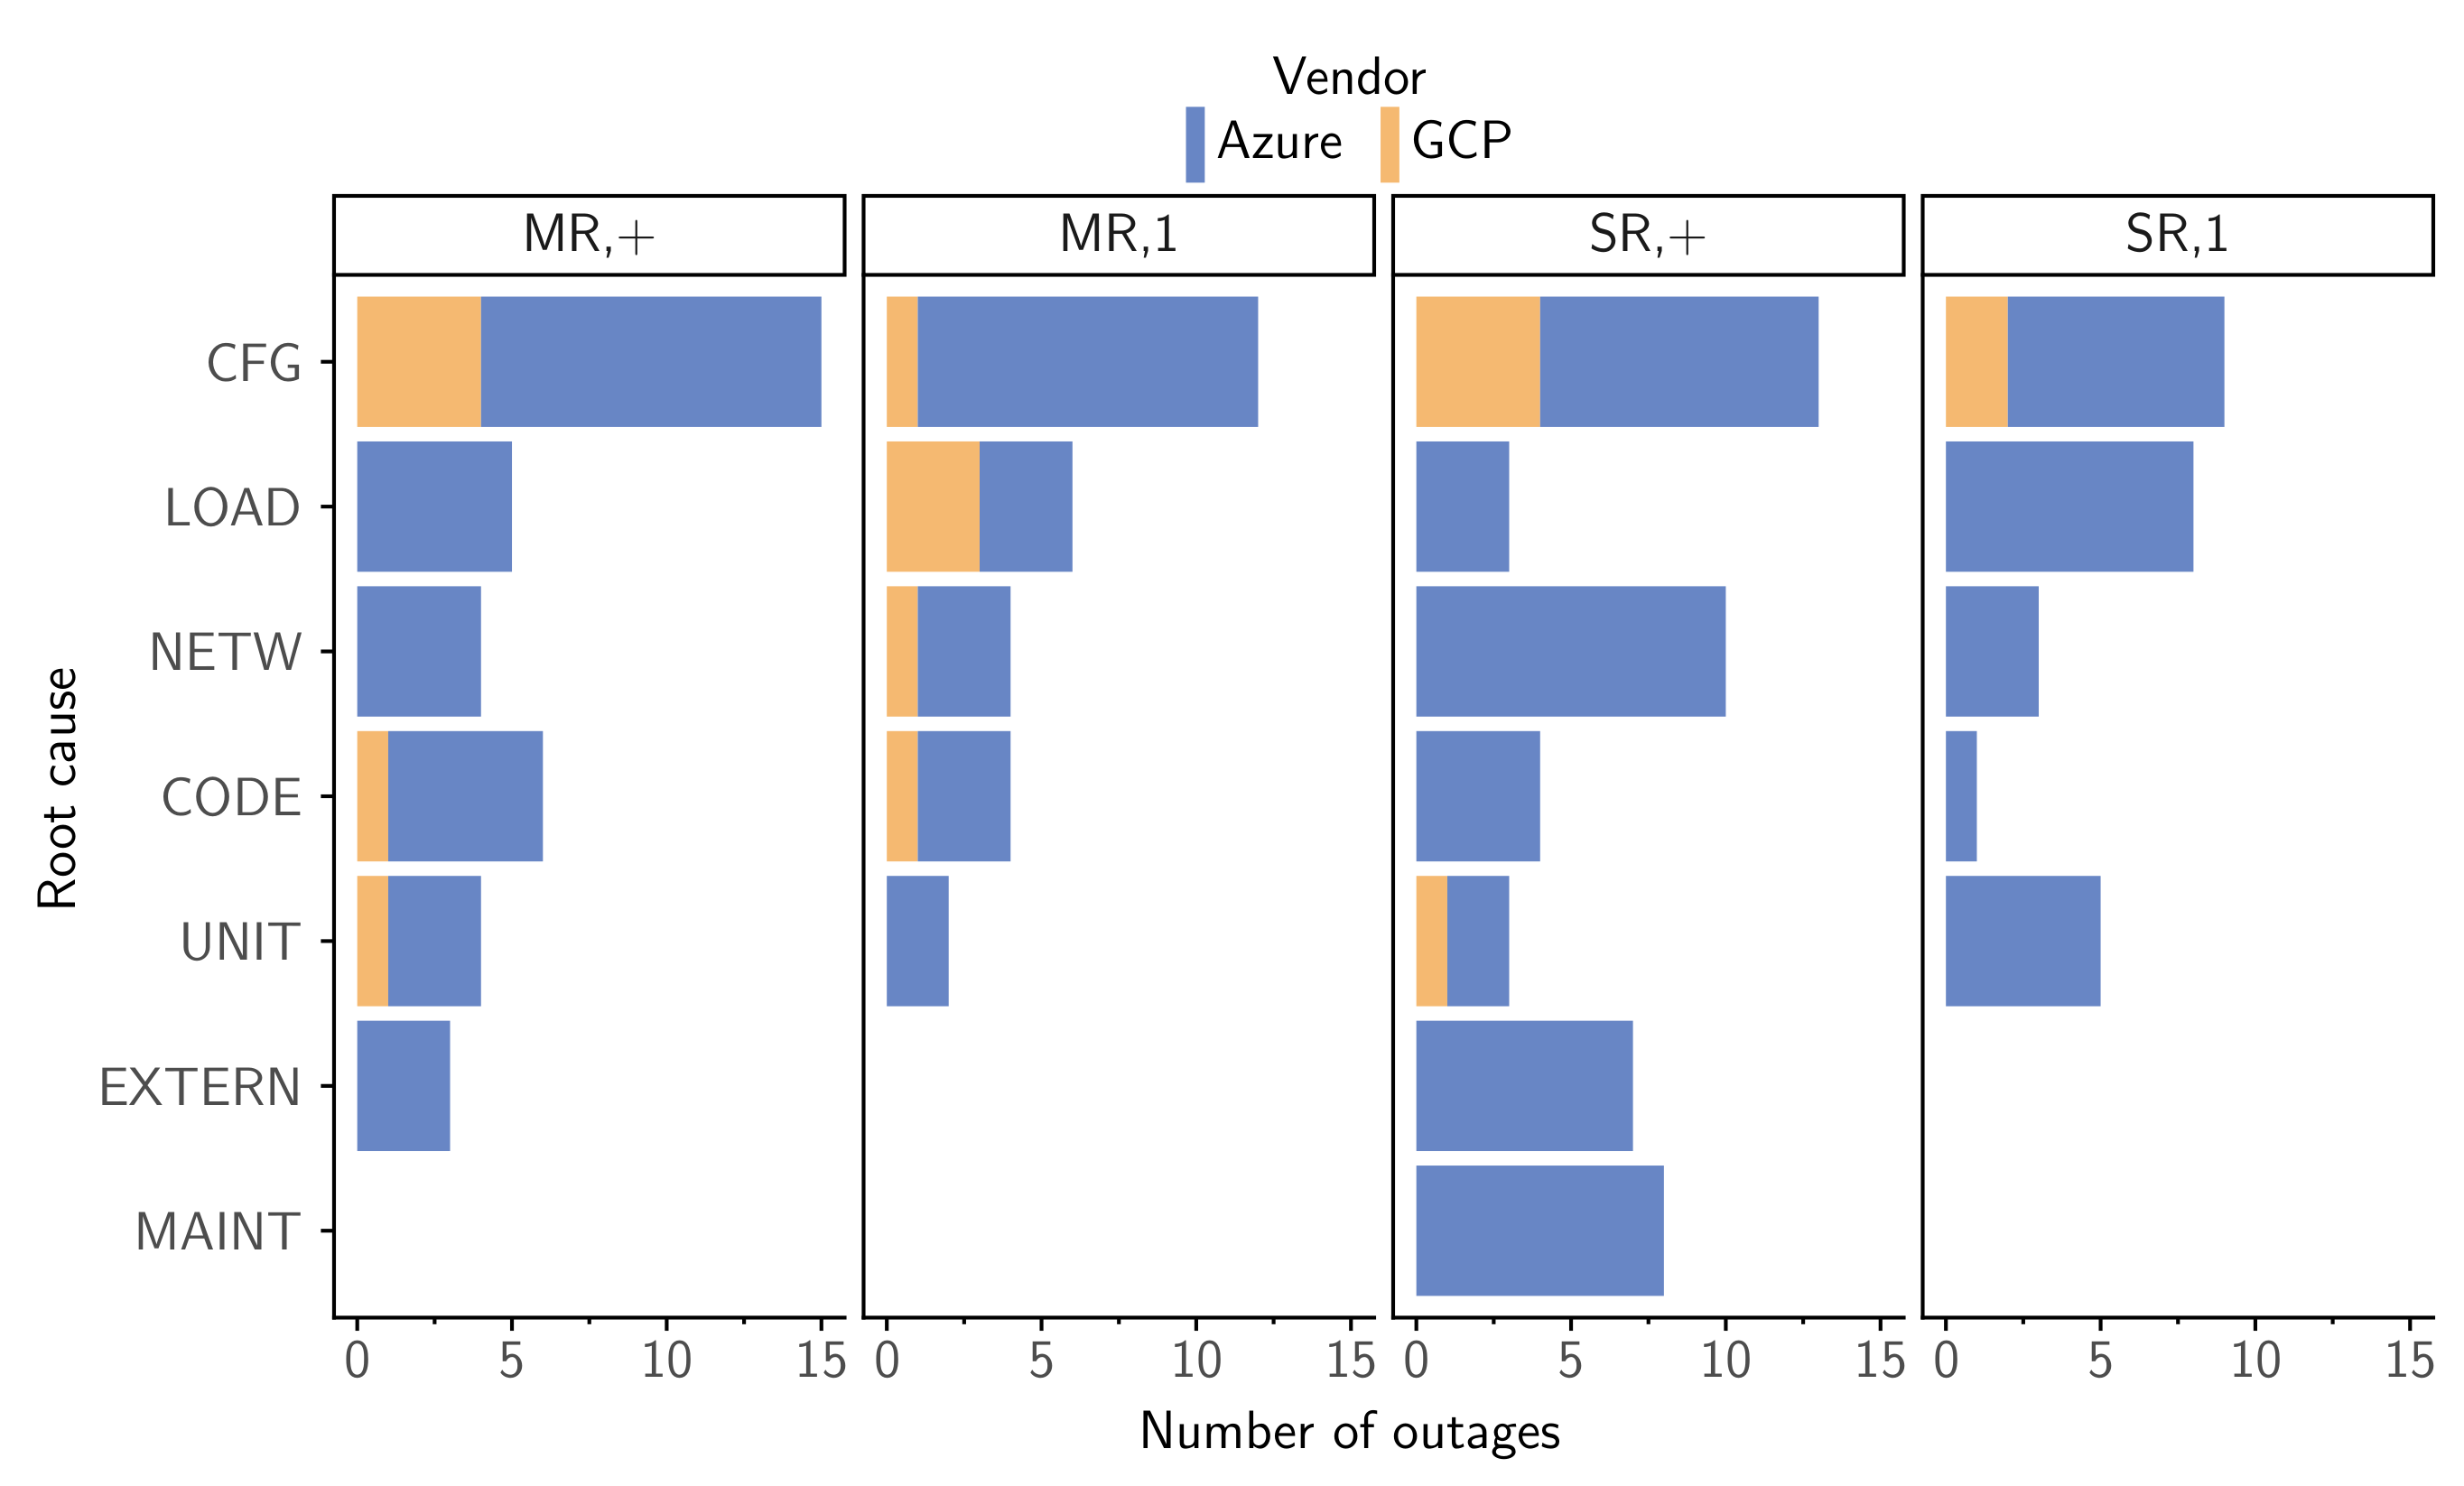
\includegraphics[scale=0.5]{root-causes-by-severity.png}
  \caption{Root causes of outages across varying severity levels, by vendor. (MR = multiple regions, SR = single region, 1 = one service, + = multiple services)}
  \label{fig:root causes by severity}
\end{figure}

We next analyse the distribution of outages across root causes and severity levels.
We identify seven classes of root causes: UNIT (individual nodes, instances, or clusters, not necessarily hardware), NETW (related to the internal or external network), MAINT (side effects caused by maintenance), LOAD (increased load on the service), EXTERN (external causes, i.e. environmental or third-party), CODE (code errors/bugs), and CFG (configuration errors).
We further separate the outages by vendor, indicated by the color of the bar in \autoref{fig:root causes by severity}.
We do not include AWS, as we do not have sufficient data regarding root causes from AWS (a cause was only specified for 2.1\% of AWS events).
Excluded from the plot are outages that did not provide a root cause (a total of \result{np-root-causes-by-severity-cause}), a range (\result{np-root-causes-by-severity-range}), or the number of affected services (\result{np-root-causes-by-severity-services}).

The majority of outages across all levels of severity are caused by configuration errors.
For multi-regional outages, the configuration category accounts for the majority by a wide margin.
On the other hand, for single-region outages, there are multiple leading causes: apart from configuration errors, outages affecting one service are also caused by increased load and failing instances, and those affecting more than one service are also caused by network errors and maintenance side effects.

\begin{figure}[h]
  \centering
  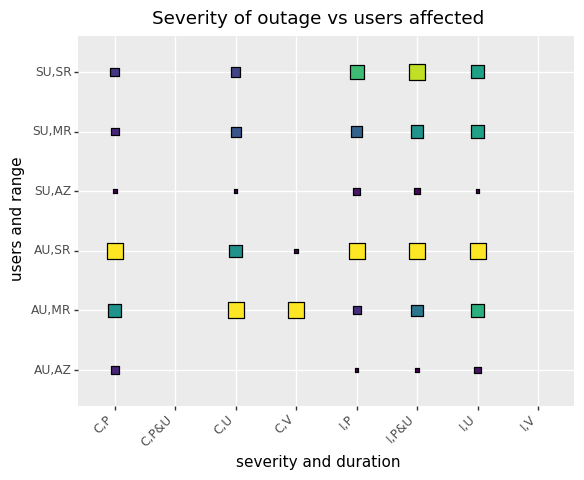
\includegraphics[scale=0.5]{severity-vs-users-affected.png}
  \caption{Severity of an outage and the users affected by the outage. (SU = some users, AU = all users, Cont = continuous, Interm = intermittent, Perf = performance degradation, Unavail = unavailable, Vis = visual)}
  \label{fig:severity vs users}
\end{figure}

Next, we consider the users affected in an outage, depending on its area of effect.
We define the area of effect of an outage as the affected users (all or some) and the range (single region or multiple regions).
We exclude events that did not state the affected users (\result{np-severity-vs-users-affected-users}), range (\result{np-severity-vs-users-affected-range}), severity (\result{np-severity-vs-users-affected-severity}), or duration (\result{np-severity-vs-users-affected-duration}).
The first immediate finding from \autoref{fig:severity vs users} is that the majority of outages result in one or more services becoming intermittently unavailable.
For outages affecting all users, in a single region or in multiple regions, there is a higher proportion of outages that cause a service to be intermittently degraded or unavailable than for outages affecting some users.
Furthermore, the majority of outages that resulted in a service being continuously unavailable (for some period of time) affected all users in multiple regions.
When the performance of one or more services is degraded, it generally happens for a continuous period of time.

\begin{figure}[h]
  \centering
  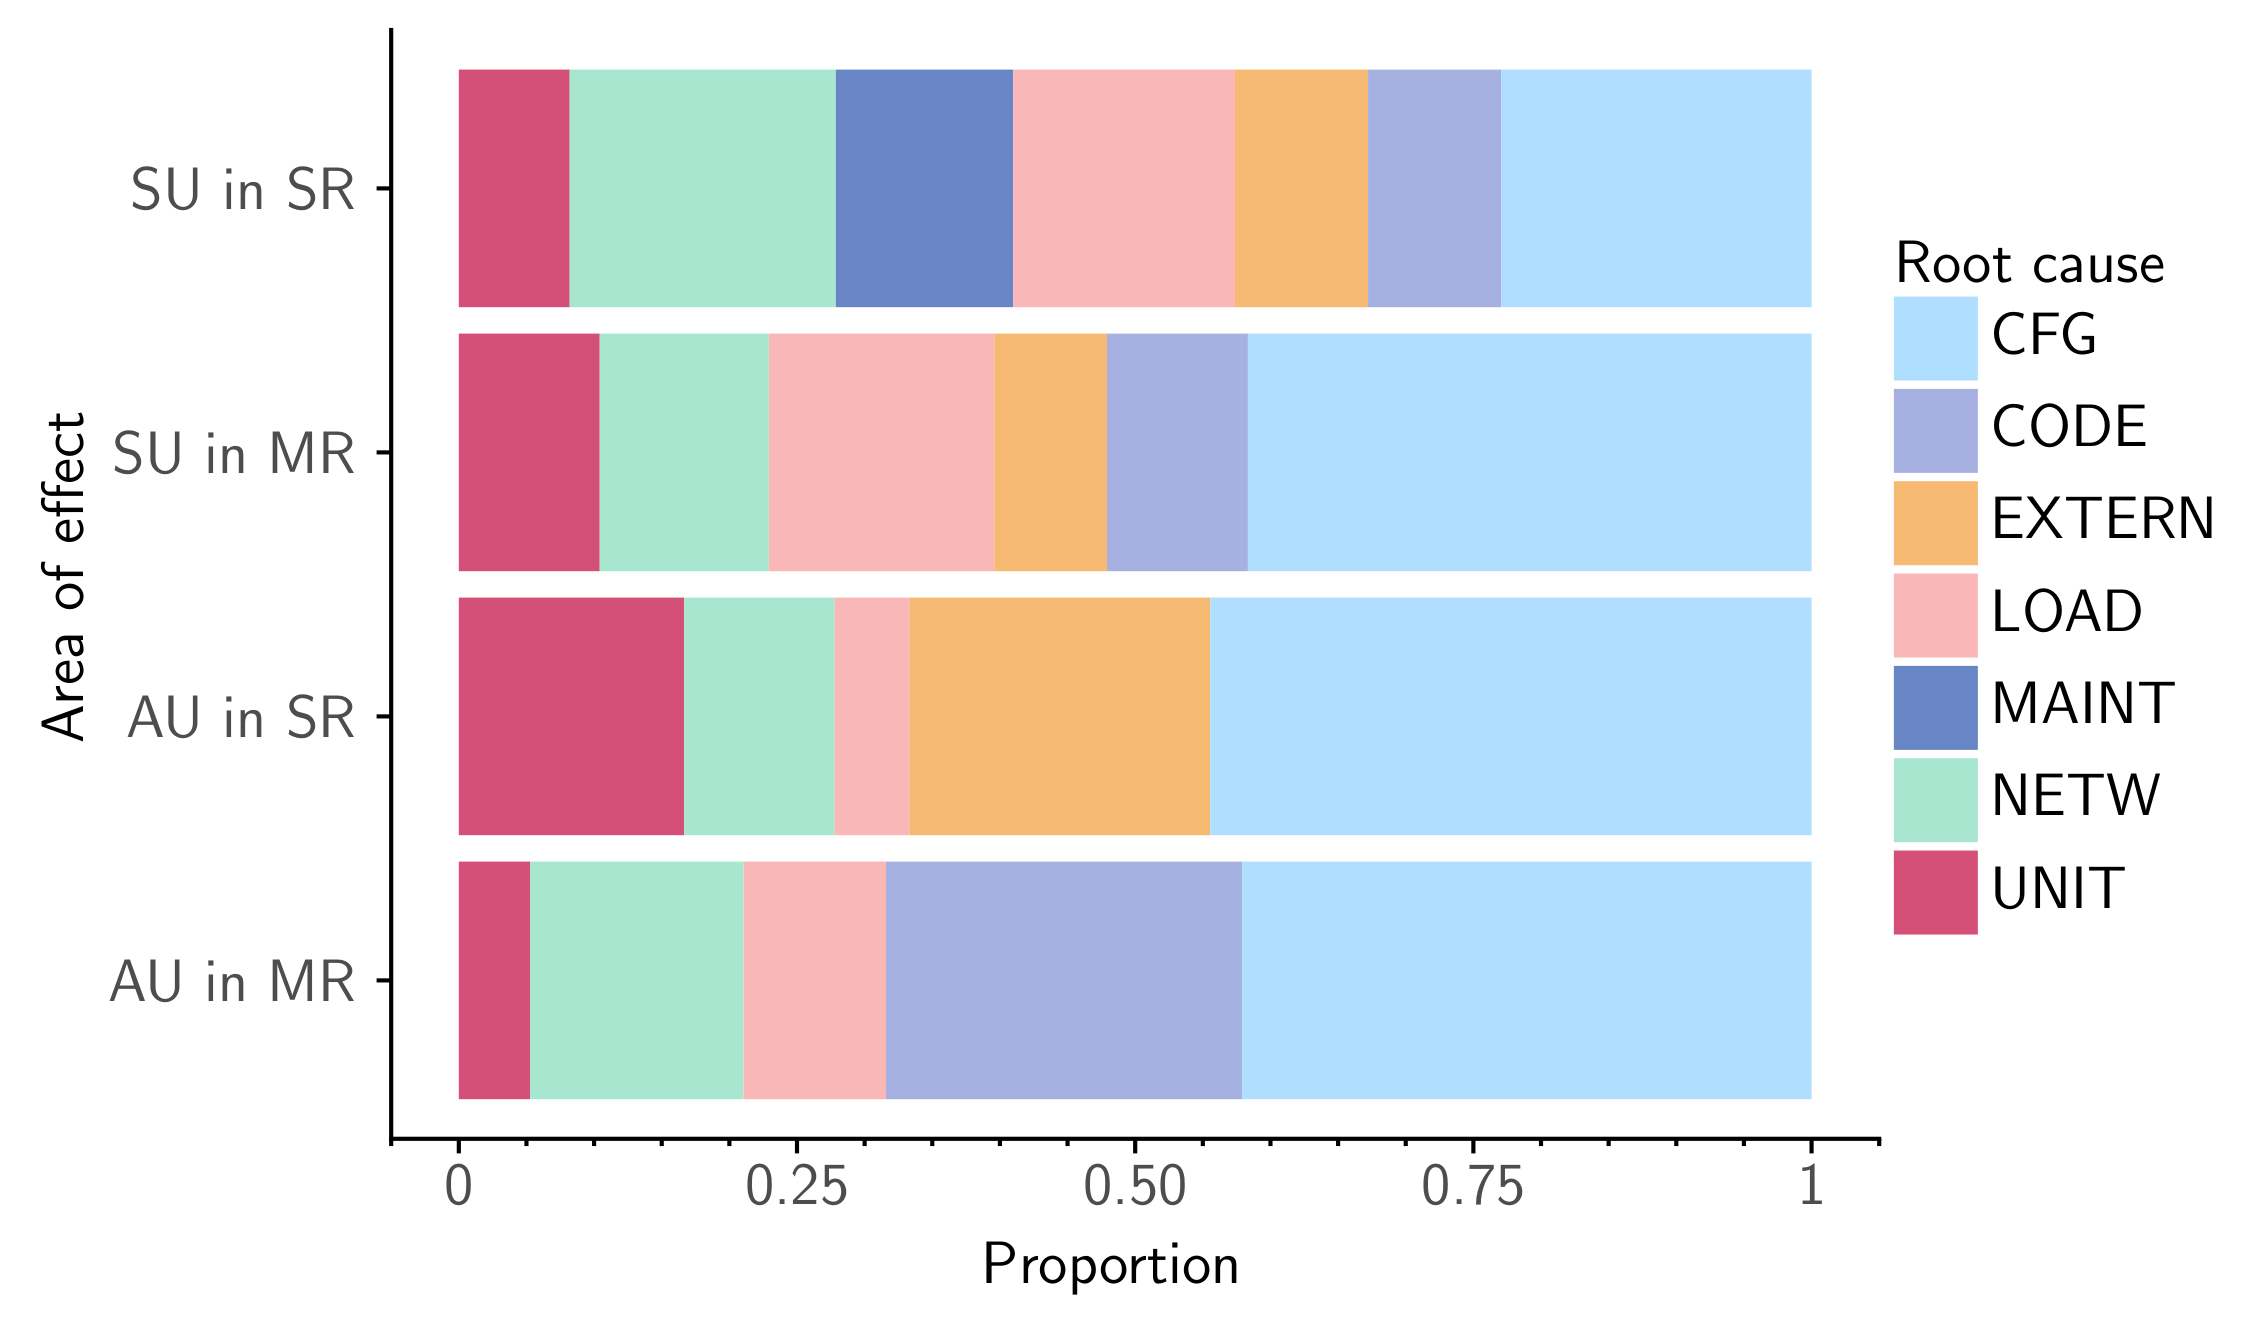
\includegraphics[scale=0.5]{range-users-vs-root-cause.png}
  \caption{Root causes of outages at various areas of effect. (SU = some users, AU = all users, SR = single region, MR = multiple regions)}
  \label{fig:causes vs aoes}
\end{figure}

We also analyze the root causes of outages, separated by the area of effect.
Here we exclude those events that did not provide a cause (\result{np-range-users-vs-root-cause-cause}), a range (\result{np-range-users-vs-root-cause-range}), or the affected users (\result{np-range-users-vs-root-cause-users}).
From \autoref{fig:causes vs aoes}, we conclude that configuration errors account for the majority of outages with the widest area of effect (all users in multiple regions).
The second main cause of such outages are code errors, which interestingly do not play a major role in single-region outages, and do not appear as a cause of single-region outages affecting all users.
Failing instances are mainly a cause of single-region outages, more so for outages that affect all users -- this is probably due to the fact that individual instances, nodes, or clusters are more localised. % TODO: requires citation or can't include this claim
From the available data, it seems that outages caused as a maintenance side effect only affect some users of the service, mostly in a single region.
It also appears that outages caused by increased load more commonly affect only some users in a given range.
The majority of outages caused by network issues affect some users in a single region, though they also play a somewhat significant role in the other area of effect categories (accounting for around 10\% of the outages in each category).

\begin{figure}[h]
  \centering
  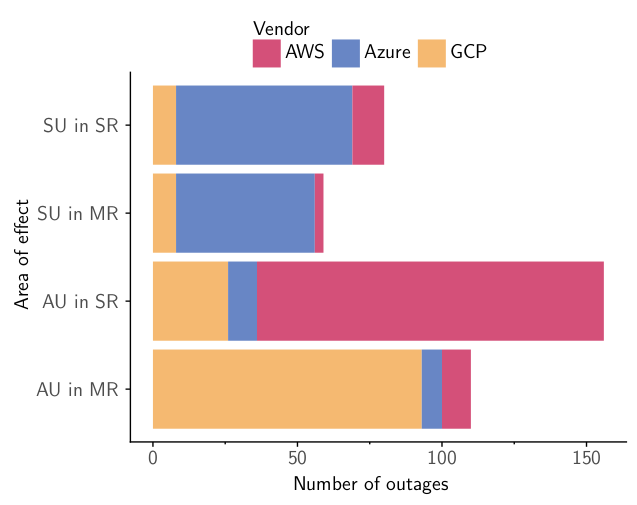
\includegraphics[scale=0.5]{users-affected-by-vendor.png}
  \caption{Area of effect of outages by vendor. (AU = all users, SU = some users, SR = single region, MR = multiple regions)}
  \label{fig:aoe by vendor}
\end{figure}

We continue with the definition of the area of effect as the affected users and the range, and analyse the distribution of outages per vendor, in figure \autoref{fig:aoe by vendor}.
We do not include events that are missing information about the users (\result{np-users-affected-by-vendor-users}) or the area of effect (\result{np-users-affected-by-vendor-range}).
We observe that the range of the majority of outages depends on the vendor.
The majority of GCP outages affect all users in multiple regions, while the majority of AWS outages affect all users in a single region.
For Azure services, the outages mostly affect some users, with an approximately equal distribution between a single region and multiple regions.

\begin{figure}[h]
  \centering
  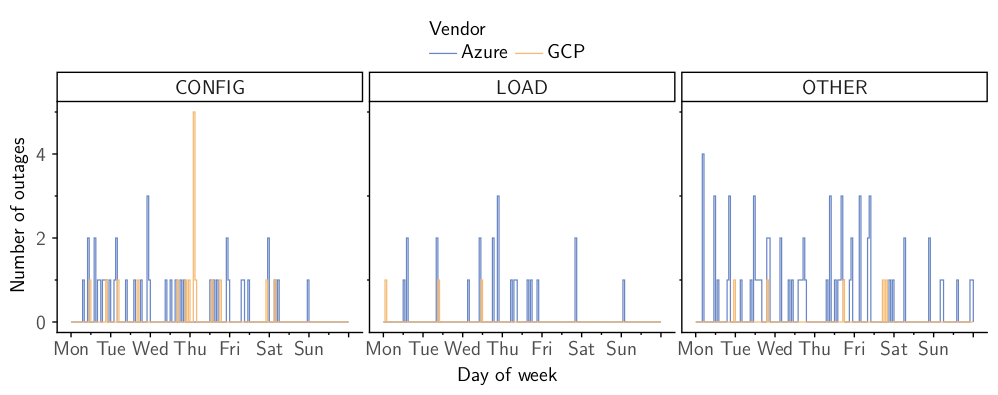
\includegraphics[scale=0.5]{causes-across-week.png}
  \caption{Outages across the week, separated by root cause and vendor. (CONFIG = configuration error, LOAD = increased load, OTHER = other)}
  \label{fig:causes across week}
\end{figure}

We also analyze the frequency of root causes at various points in the week, separated by vendor.
We do not include AWS outages here, due to a lack of specified root causes.
Outages that did not provide a root cause are also excluded (\result{np-causes-across-week-cause}).
From \autoref{fig:causes across week}, it seems that load-related outages tend to happen starting between midday on Wednesday and Thursday evening, with smaller peaks during the night on other days.
Most outages caused by misconfiguration happen in the first half of the week, from mid-Monday until midnight on Thursday.
This could perhaps be because large code changes are usually introduced during the first few days of the week. % TODO: claim needs supporting
The major peaks for these outages generally occur around midnight; the reason for this could be that deployments happen during the night, when it is likely that fewer customers will be using the service. % TODO: need a source here
Outages related to other root causes generally occur during the weekdays, and there are only a few peaks during the weekend.
It is important to note here that this is a relatively small dataset, and the trends observed in \autoref{fig:causes across week} could change if more data becomes available.

\begin{figure}[h]
  \centering
  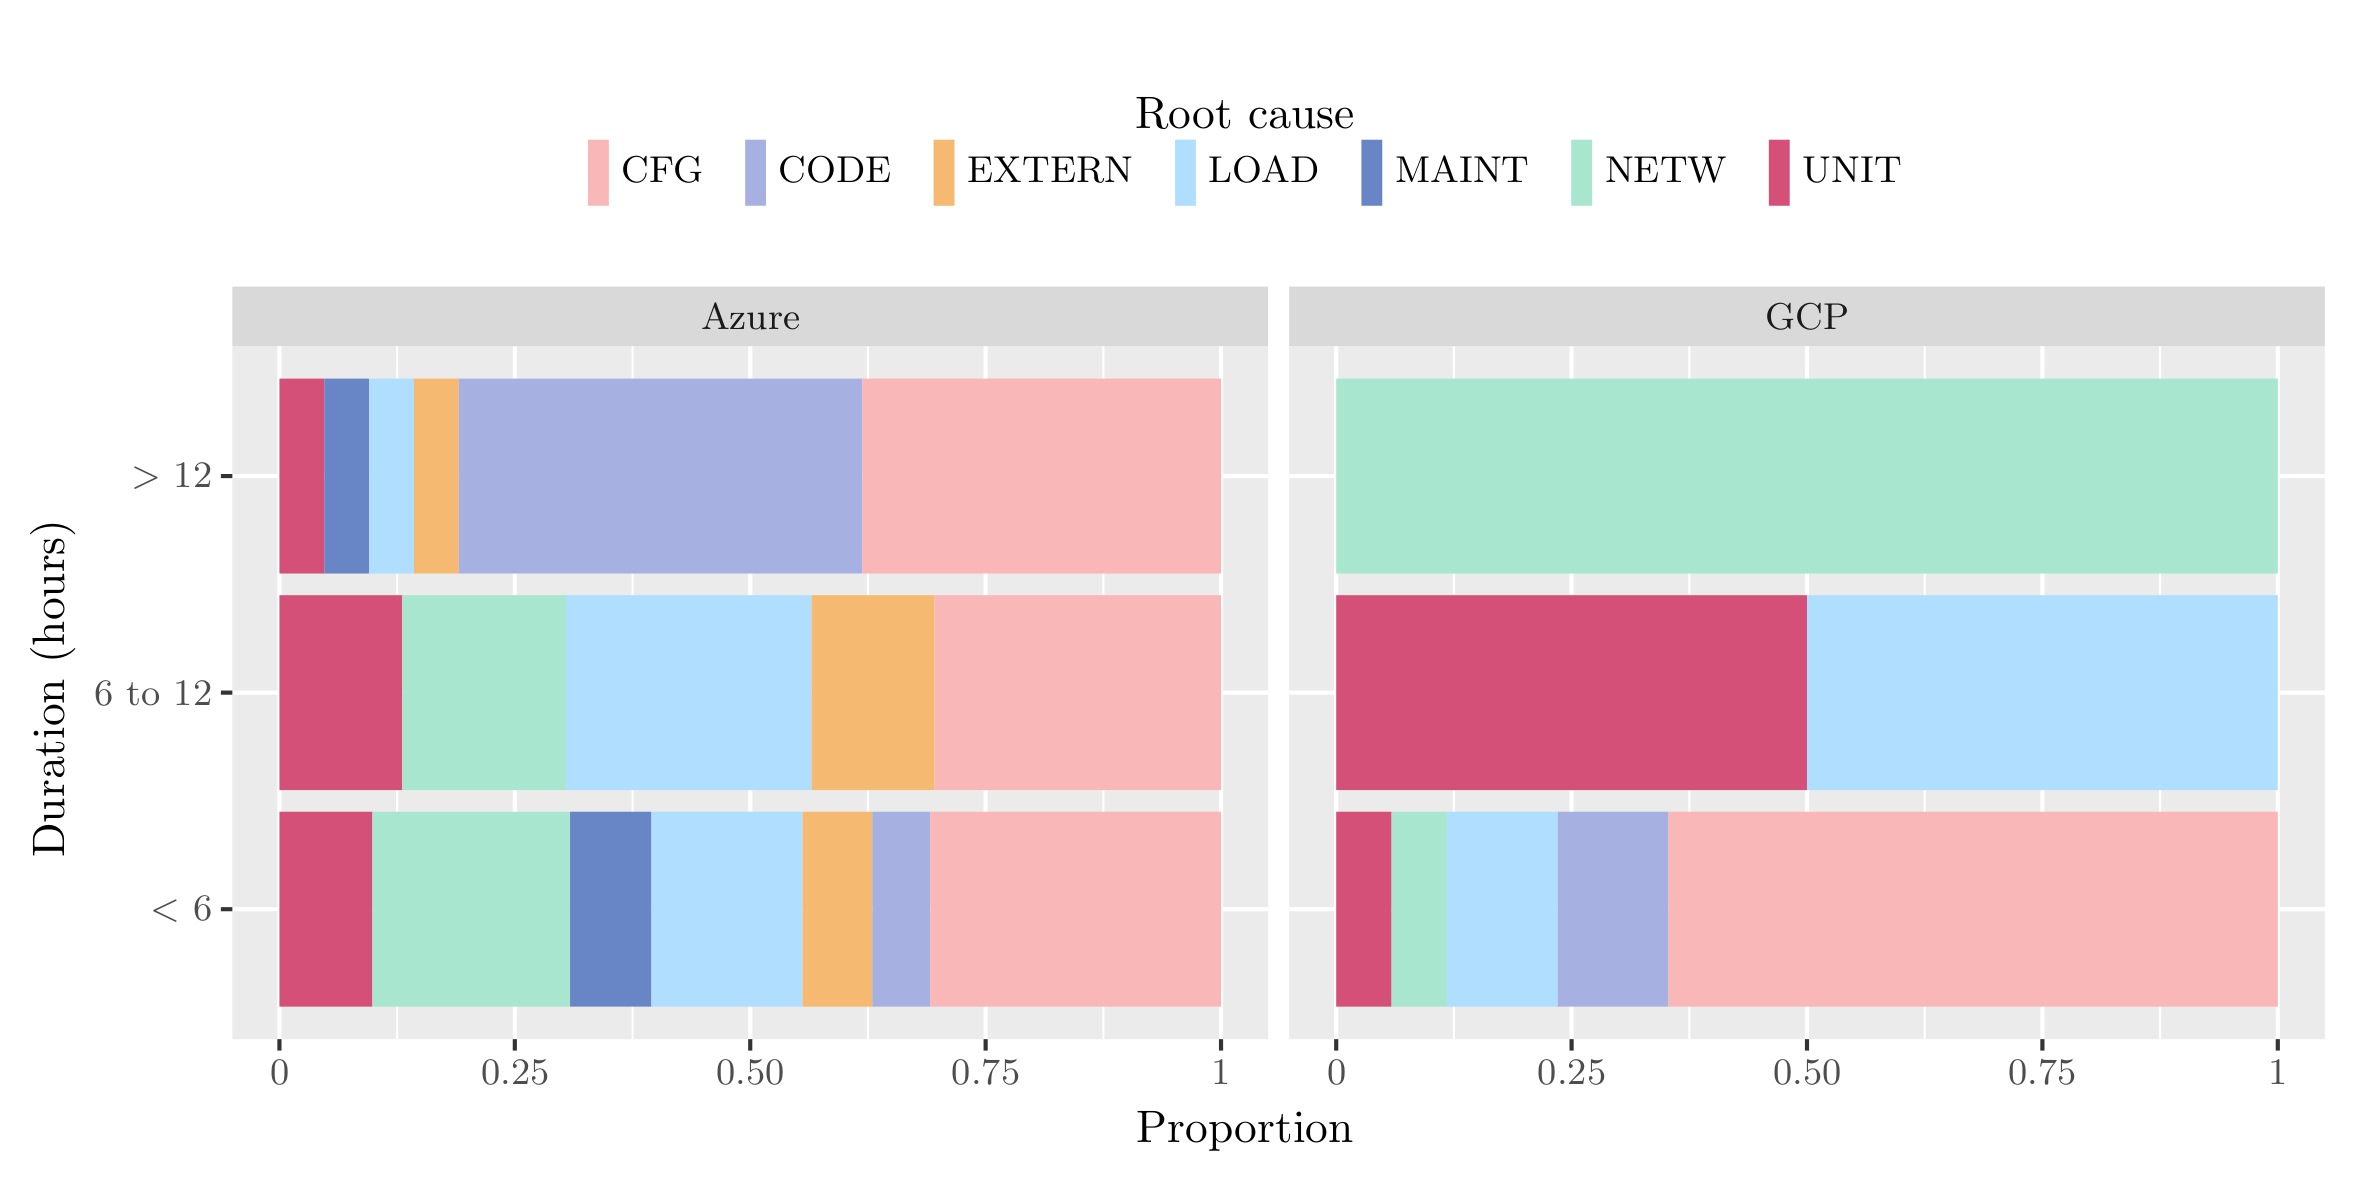
\includegraphics[scale=0.5]{causes-vs-duration-hr-ranges.png}
  \caption{Root causes of outages, separated by duration and vendor.}
  \label{fig:causes vs duration ranges}
\end{figure}

We separate the outages by duration, in three categories: short (outages lasting less than six hours, '< 6'), medium (six to twelve hours '6 to 12'), and long (more than twelve hours '> 12').
The outages are grouped by duration and vendor, such that the horizontal axis shows the proportion of outages for a specific duration category and vendor.
We do not plot outages that did not specify a root cause (\result{np-causes-vs-duration-hr-ranges-cause}).
All AWS outages that specified a cause were shorter than six hours, and were caused by external events (e.g. third party or environment).
However, as discussed above, only three AWS outages specified a cause, so AWS is not included in \autoref{fig:causes vs duration ranges}.
Azure services have more diverse outage causes than GCP services.
All outages of GCP services that lasted longer than twelve hours were caused by network errors; in contrast, network errors did not play a role in these types of outages for Azure services.
The longest outages of Azure services were caused in approximately equal parts by code errors, and by configuration errors.
Configuration errors were a common cause of Azure outages for all three duration categories, while only the shortest GCP outages (shorter than six hours) had configuration errors as a cause.
For both GCP and Azure, increased load was a main factor in the short- and medium-duration outages.
For GCP, there were more medium-duration outages caused by increased load than short-duration outages; for Azure services, the proportion is approximately the same.
GCP also had failing computational units as a major cause for medium-duration outages; this was not as prominent for Azure services, where failing units accounted for approximately the same proportion of short-duration outages as for medium-duration outages.

\begin{figure}[h]
  \centering
  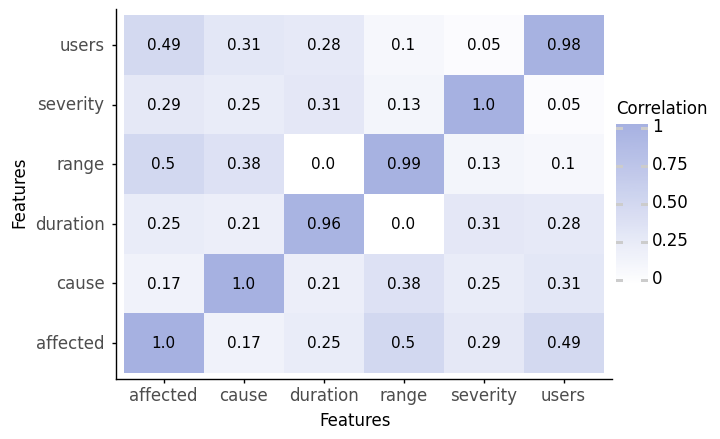
\includegraphics[scale=0.5]{cramers-v.png}
  \caption{Cram\'{e}r's V matrix}
  \label{fig:cramers v}
\end{figure}

Finally, we conduct correlation analysis on the various features of the data.
The first statistic we consider is Cram\'{e}r's V, which measures association between two nominal variables.
% TODO: information about Cramer's V and reasoning for choice, properly cited
Applying the measure to the dataset, we obtain a correlation matrix shown in \autoref{fig:cramers v}.
We observe that there is no strong correlation between any of the features.
Relative to the other values in the matrix, the component affected in the outage seems to be moderately correlated with the range of the outage (0.5), and with the users affected in the outage (0.49).
There may also be a slight correlation between the cause of the outage and the range of the outage (0.38), as well as with the users affected in the outage (0.31).
However, since the values are low, these results are inconclusive.

\begin{figure}[h]
  \centering
  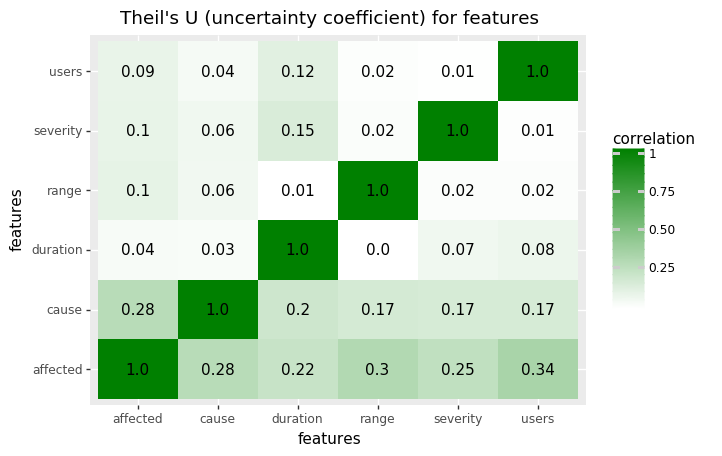
\includegraphics[scale=0.5]{theils-u.png}
  \caption{Uncertainty coefficient matrix (Theil's U)}
  \label{fig:theils u}
\end{figure}

We also calculate uncertainty coefficients, also known as Theil's U, for the features of the data; this is shown in a matrix in \autoref{fig:theils u}.
% TODO: more information about uncertainty coefficient and reasoning for choice, cited properly
The results show no clear association, as the coefficients are low.
However, the users affected in the outage could determine the affected component (0.34) and range of the outage (0.3).
This seems to support the findings from \autoref{fig:cramers v}.
Similarly, the affected component could determine the cause of the outage (0.28).
